\section{Implementación}
La implementación de los diversos algoritmos y estructuras de datos fue realizada en el lenguaje de programación C. Las diferentes funciones y estructuras fueron implementadas en archivos separados, con el objetivo de mantener una estructura de directorios clara y ordenada. A continuación se detallara esta implementación.

\subsection{Estructura de directorios}
Dentro del directorio \texttt{src} se encuentran los siguientes archivos:
\begin{itemize}
    \item \texttt{BuddySystem.c}: Contiene la implementación del algoritmo de asignación de memoria Buddy System.
    \item \texttt{errors.c}: Contiene la implementación de funciones para manejar errores.
    \item \texttt{files.c}: Contiene la implementación de funciones para manejar archivos.
    \item \texttt{forking.c}: Contiene las funciones para manejar \texttt{main} dentro del programa, utilizando las demás funciones y estructuras del proyecto.
    \item \texttt{main.c}: Contiene la función \texttt{main} del programa.
    \item \texttt{process.c}: Contiene la implementación de funciones y estructuras de datos para manejar procesos.
    \item \texttt{queue.c}: Contiene la implementación de funciones y estructuras de datos para manejar colas.
    \item \texttt{utilities.c}: Contiene la implementación de funciones varias, de utilidad.
\end{itemize}

Dentro del directorio \texttt{testing}, se encuentran los archivos:
\begin{itemize} 
    \item \texttt{generator.c}: Contiene la función encargada del generador de ``procesos''.
    \item\texttt{gant\_creator.py}: Es un script de \textbf{Python} encargado de generar una carta gantt.
\end{itemize}
Por ultimo, dentro del directorio \texttt{incs} se encuentran las cabeceras incluidas en todos los archivos \texttt{.c}.


\subsection{Estructuras de datos}
Las estructuras de datos utilizadas fueron las siguientes:
\subsubsection*{Lista enlazada simple}
Esta se encuentra implementada con la estructura \texttt{ProcessNode}, el cual contiene las variables:
\begin{itemize}
    \item \texttt{Process data}: Donde se almacenarán los procesos
    \item \texttt{Position next}: Puntero al nodo siguiente de la lista
\end{itemize}
La lista enlazada simple se utilizo para almacenar y ordenar los procesos ingresados en el programa según su \textit{arrival time}, el ordenamiento de la lista se realizo en primer instancia con \textit{bubble sort}, sin embargo al probar el programa en cantidades grandes, lo ineficiente de este algoritmo salio a flote, debido a que se encontró con tiempos de espera extensos al ejecutar el programa. A raíz de de esto se decidió implementar el algoritmo \textit{merge sort}, el cual redujo sustancialmente la cantidad de tiempo de demora del programa en ordenar los datos.

Esta estructura de datos es la encargada de almacenar los procesos en memoria, con esto las demás estructuras unicamente deben utilizar punteros a estos datos, ahorrando una cantidad significativa de espacio.

\subsubsection*{Colas}
Las colas se encuentran implementadas con la estructura \texttt{CircularNode}, la cual, en realidad es una \textit{lista circular doblemente enlazada} en donde el \textit{rear} y el \textit{front} de la cola son representadas por el nodo anterior y siguiente del centinela de la lista. Este contiene las variables:
\begin{itemize}
    \item \texttt{Process* process}: Puntero al proceso almacenado. Este puntero apunta a algún proceso contenido en la lista enlazada simple anterior
    \item \texttt{PtrToCircularNode next}: Puntero al nodo siguiente de la lista
    \item \texttt{PtrToCircularNode prev}: Puntero al nodo anterior de la lista
\end{itemize}

La implementación de las colas fue fundamental para el funcionamiento del programa, ya que sus características permiten manejar fácilmente el flujo y orden de los procesos. Las colas fueron usadas en el:
\begin{itemize}
    \item Arrival Queue
    \item Waiting Queue
    \item SJF
    \item RoundRobin
\end{itemize}


Para insertar elementos en las colas existe la función estándar de \texttt{enqueue}, la cual simplemente ingresa un elemento en la cola, sin embargo por motivos de comodidad y para cumplir con el funcionamiento deseado se incluyo la función \texttt{sorted\_enqueue}, la cual se encargo de ingresar decreciente o crecientemente  un proceso en cola según un criterio dado. Por ejemplo al ingresar en  SJF se ingresa según su \textit{burstime}.

\subsubsection*{Arboles binarios}
Los arboles binarios se encuentran implementados en la estructura \texttt{\_treeNode} , definida por las siguientes variables:
\begin{itemize}
    \item \texttt{Buddy element}: Corresponde  a una estructura la cual contiene un puntero a proceso, la altura del elemento dentro del arbol y una banera que indica el estado de uso del elemento, representadas por: \texttt{Process* process}, \texttt{unsigned int order} y \texttt{isUsed} respectivamente.
    \item \texttt{TreePosition parent}: Puntero a nodo el cual representa al nodo padre.
    \item \texttt{TreePosition left}: Puntero a nodo que representa al hijo izquierdo.
    \item \texttt{Treeposition right}: Puntero a nodo que representa al hijo derecho.
\end{itemize}

El árbol binario fue implementado en el \textit{BuddySystem},  asignando ``memoria'' inteligentemente mediante el operaciones relacionadas a las potencias de dos y logaritmos en base dos, con el fin de decidir el espacio optimo del proceso entregado según su memoria requerida. Inicialmente estas operaciones se realizaron matemáticamente, mediante funciones de la biblioteca \texttt{math.h} sin embargo se opto por realizarlas de forma binaria, lo que disminuyo la carga del programa, haciéndolo mas eficiente.


\subsection{Algoritmos de planificacion}
Como ya fue mencionado anteriormente los algoritmos de planificación utilizados fueron \texttt{Shortest Job First y Round Robin}. Su implementación consistió en:

\begin{itemize}
    \item \textbf{Shortest Job First}: Para la implementación del algoritmo \textit{SJF} se utilizo una cola a través de una lista circular doblemente enlazada, esta cola se ordeno mediante la función \texttt{sorted\_enqueue}, realizando comparaciones con el \textit{burstime} del proceso que esta siendo trabajado (en caso de que la cola que este siendo procesada sea \textit{SJF}) con el proceso ingresado.

    \item \textbf{Round Robin}: En el caso de la cola \textit{Round Robin}, esta se trabajó con la misma estructura de datos que el \textit{SJF}, sin embargo el funcionamiento de esta consiste en revisar el \textit{burstime} del proceso a ser trabajado, se realiza una comparación para ver si es igual o mayor que el \textit{Quantum}, de ser asi se asigna a esta cola y este proceso es trabajado la cantidad de ticks que indica el \textit{Quantum}. Al llegar al final del \textit{Quantum} se verifica si el proceso debe pasar o no a la cola \textit{SJF} mediante una comparación simple.
\end{itemize}

\subsection{Otros ejecutables}

Otros programas utilizados en la ejecución del programa fueron un generador de procesos y parámetros y un generador de carta gant. El primer programa corresponde a un generador simple de procesos, el cual entrega parámetros aleatorios entre ciertos valores dados por el usuario mediante terminal.

\lstinputlisting[caption=Ejemplo de entrada forKing, label={lst:exampleInput}]{src/input.txt}


Mientras que el generador de carta Gantt utiliza el lenguaje de programación \textbf{Python} con las librerias \texttt{matplotlib, numpy y random}, leyendo un archivo tipo csv el cual se genera al ejecutar el programa principal.

\begin{figure}[!ht]
    \centering
    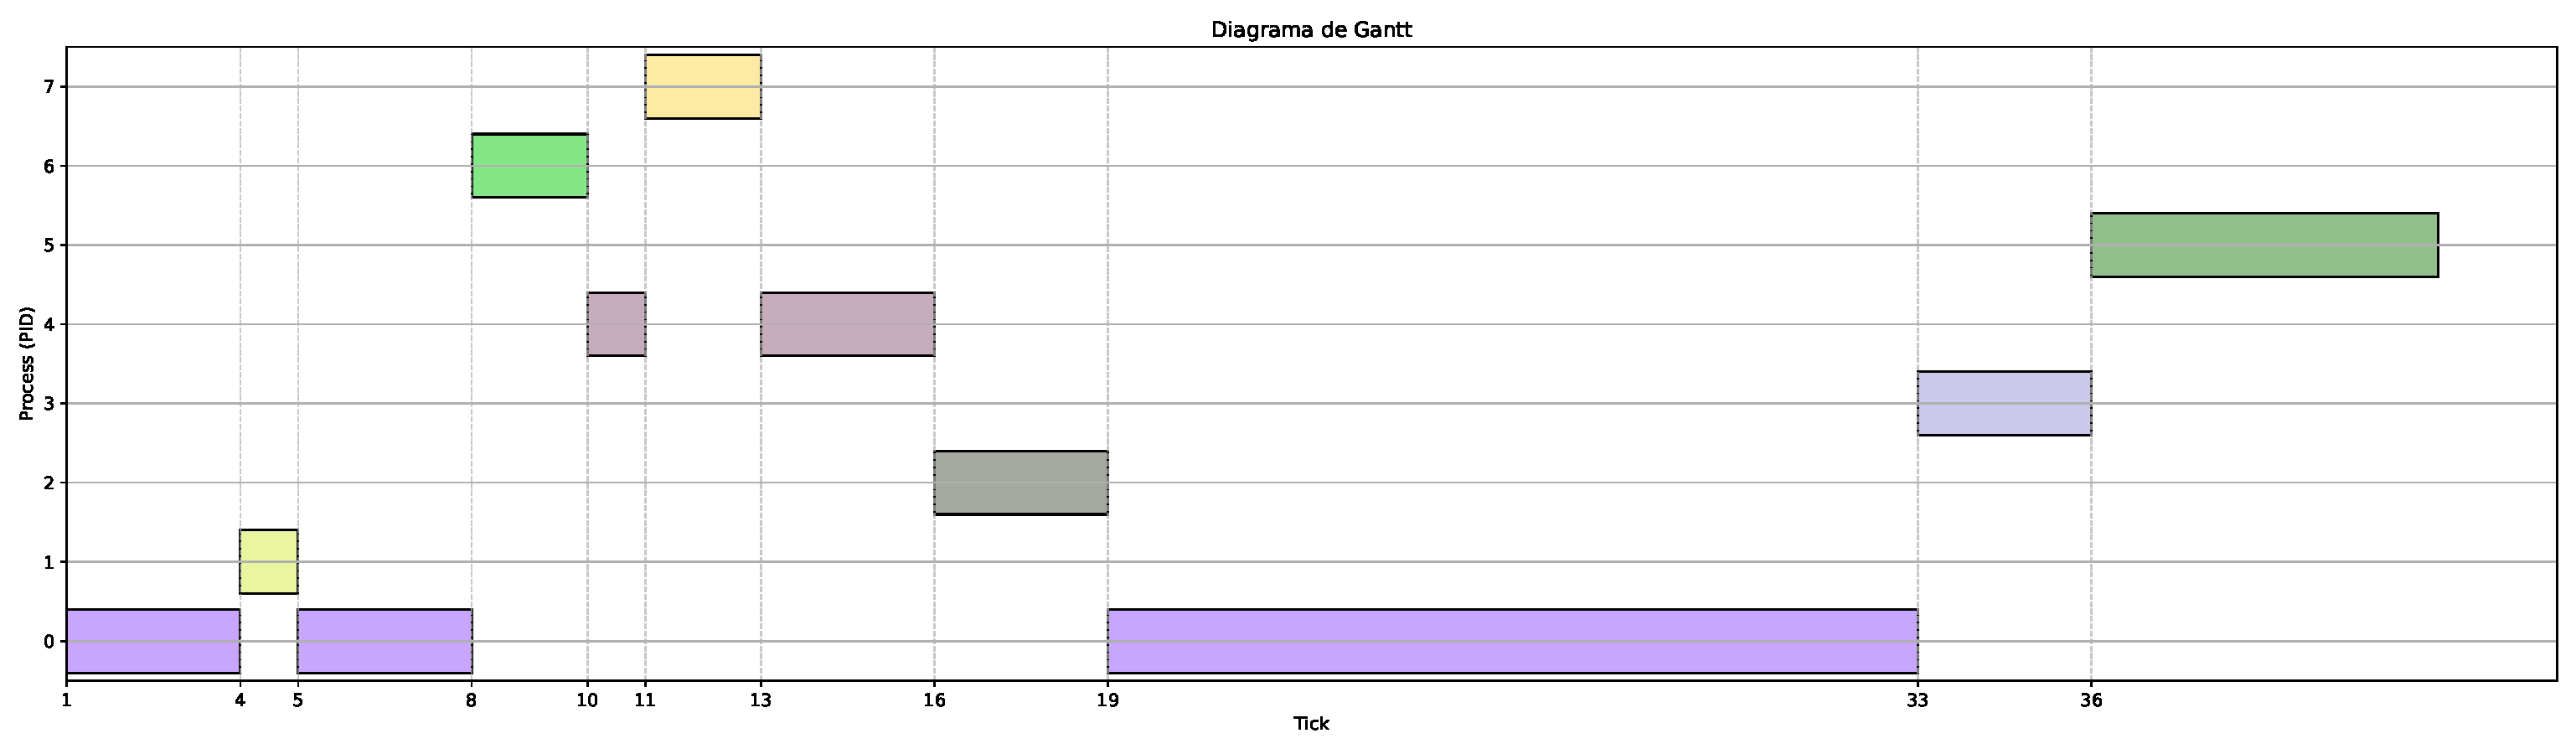
\includegraphics[width=\textwidth]{src/figures/carta_gant.pdf}
    \caption{Ejemplo de carta Gantt con forKing}\label{fig:gantt}
\end{figure}